\documentclass{article}
 %\usepackage{suthesis-2e}
\usepackage{amsmath}
\usepackage{amsthm}
\usepackage{amsfonts}
\usepackage{algorithm}
\usepackage{algpseudocode}
\usepackage{graphicx}
%Set up plotting stuff
\usepackage{pgfplots}
%\usepackage{showkeys}
\usepackage{verbatim}

\begin{document}
\newcommand{\X}{\mathcal{X}}
\newcommand{\T}{\mathcal{T}}
\newcommand{\bigO}{\mathcal{O}}
\renewcommand{\Re}{\mathbb{R}}
\newcommand{\pmat}[1]{\begin{pmatrix}#1\end{pmatrix}}

\title{Notes on sparse direct methods}
\maketitle

\section{Definitions}
\subsection{Undirected graph of a symmetric matrix}

Let $A\in \Re^{n\times n}$ be a matrix. The undirected 
graph of $A$ denoted $G_A=\left\{ V,E \right\}$ is defined by the set of 
nodes $V = \left\{ 1,\cdots,n \right\}$ and 
edges $E = \left\{ (j,i) \mid A_{i,j} \neq 0 \right\}$. 

\subsection{Filled graph of $A$}
If we calculate the Cholesky factorization $A=LL^T$ of a symmetric positive matrix or
the $A=LDL^T$ factorization of a strongly quasi definite matrix, the non zero pattern 
of $L$ will be the same. 
The filled graph of $A$ is the graph $G_{L+L^T}$.

\subsection{Directed graph of $L$}
For a lower triangular matrix $L\in\Re^{n\times n}$ we define the directed
graph $G_L$ as follows: $V = {1,\dots,n}$ and $E = \left\{ (j,i) \mid L_{i,j}
\neq 0 \right\}$

The node corresponding to column $j$ is a child of all the non zeros in column
$j$.  Because the matrix is lower triangular all parents have larger index
than the parent and the graph is acyclic. \cite[Page 30]{Sparse Davis}

\subsection{The reach of a set}
The reach of a set $B$ denoted $\operatorname{Reach}(B)$ is the set of 
all nodes reachable from the nodes in $B$ in the directed graph $G_L$.
That is, the set of all nodes $i\in V$
such that there exists a $j \in B$ and a path $j \to i$ in $G_L$.

\subsection{The nonzero pattern in $x$ when solving $Lx=b$}
    Sparse solves with lower triangular matrices achieve assymptotic 
    solve times that can be potentially less than $\bigO(n)$. This is only possible because 
    the algorithm does not have to visit all entries of $x$ (just visiting them 
    implies order $\bigO(n)$ operations).

\subsection{Eliminiation tree}
    The elimination tree $\T(A)$ (denoted $\T$ for short) 
    defines the order in which the columns of 
    $A$ have to be processed to build $L$. For example the tree given by 
    \eqref{tree:A} indicates that 2  3 and 1 have to be processed before four, 
    it also indicates that 2 and 3 can be processed at the same time as 1 is processed, 
    and defines the first level of parallelism that can be achieved. 
\begin{figure}[H]
\centering
    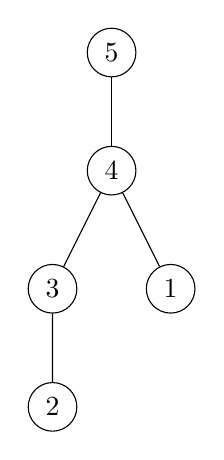
\begin{tikzpicture}[scale=1]
             \node[circle,draw]{5} child {
                                   node[circle,draw]{4} child{
                                                         node[circle,draw]{3} 
                                                         child{node[circle,draw]{2}}}
                                                         child{node[circle,draw]{1}}
                                                         };
    \end{tikzpicture}
\caption{Elimination tree of $A$}
\label{tree:A}
\end{figure}

The elimination tree $\T$ is in fact a forest, but we use the term tree for simplicity. 
The elimination tree $\T$ of $A$ is defined from the nonzero pattern of the Cholesky factor $L$ as follows:
Each node $i$ has as parent the first nonzero sub diagonal in column $i$ of $L$. 
For example if the 3rd column of $L$ has pattern \[\pmat{o\\o\\x\\o\\x\\o\\x}\] then 
the parent of 3 is 5. 
It is clear that this defines a tree since each node can only have one parent
and each parent can only have a higher index. 
The roots of the tree are the set of columns of $L$ which have only zeros 
below the diagonal. \\

Why is this tree in fact the dependency graph follows from the next observation:
When column $i$ is eliminated, all the non zeros bellow the diagonal will form
a clique in the elimination graph.
For example when 3 is eliminated from the
above pattern, the outer product  \[\pmat{o \\ x\\ o \\ x} \pmat{o & x & o & x} = \pmat{ o &
o & o & o\\ o & x&o&x\\o &o&o&o\\o&x&o&x}\] will be subtracted from the remaining matrix. This
will induce non zeros in columns 5 and 7, particularly column 5 will now have
non zeros, wherever it allready had in addition to the non zeros of column 3.
In a loose sense column 5 inherits all the non zeros of column 3.

The elimination of column 3 affected all columns where it had non zeros bellow the diagonal, namely 
5 and 7, however because 5 *inherits* all the non zeros, it will affect the same columns 3 affected. 
For all of those columns following 5 (namely 7) we dont have to worry about the dependency with column 
3 for the elimination of column 5 will induce the same zeros and more. Therefore a columns parent 
is the first column it will create fillin at, or the first nonzero bellow the diagonal.

A fast algorithm to compute $\T$ from $A$ is given by Tim Davis.

\section{Supernodal cholesky}
From here on im fuzzy on the details

\subsection{Supernodal tree}
The idea behind supernodal algorithms is to group nodes from the tree to create a coarser 
tree. Each grouping is a super node, each super node is processed as a block using dense 
algebra, thus winning speed trough the data reuse dense algebra induces and allowing for 
parallelism between blocks. 
Returning to the example of \eqref{tree:A}, the grouping of 2 and 3 into a node and 4 and 5
forms the super node tree \eqref{tree:superA}.
\begin{figure}[H]
\centering
    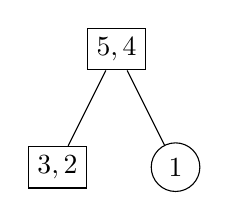
\begin{tikzpicture}[scale=1]
             \node[draw]{$5,4$} child{node[draw]{$3,2$}}
                                     child{node[circle,draw]{1}};
                                                        
    \end{tikzpicture}
\caption{Elimination tree of $A$}
\label{tree:superA}
\end{figure}

\subsection{Permutations of the matrix that yield the same elimination tree}
Just my intuition
First some observation about the numbering of the nodes in elimination trees:
all descendents of a node have smaller indices and all predecessors have larger numbers, 
on the other hand all children have larger. 
Permuting $A$ in such a way that this property is maintained for a fixed tree, yields the 
same elimination pattern\dots


\subsection{Block algorithm}
Assume we permute the matrix to the ordering $P = (3,2,1,4,5)$
the elements of a leaf supernode to form the matrix 
\[\hat A = \pmat{A_{3,2}          & 0            & A_{(3,2),(4,5)} \\
                 0                & A_{1}        & A_{1,(4,5)}\\
                 A_{(3,2),(5,4)}^T& A_{1,(5,4)}^T& A_{(4,5),(5,4)} }
                 \]


%\subsection{Row subtree}
%We define a nested family of elimination trees $\T_k$ in the following way:
%$\T_k$ is the elimination tree of the upper triangular section of $L$ formed
%from its first $k$ rows and columns, i.e. $\T_k$ is the elimination tree of
%$L_k = L(1:k,1:k)$.  To see that the trees form a nested family, observe that
%appending row $k+1$ of $L$ to $L_k$ forms $L_{k+1}$. From this operation only
%roots of $\T_k$ can acquire node $k+1$ as a parent. Furthermore
%the roots of $\T_k$ that acquire a new parent are those corresponding to a non
%zero of row $k+1$ of $L$.
%
%\section{Solving with sparse RHS}
%Assuming that $L$ has non-zero diagonal (equivalently that $L$ is of full rank), 
%then the non zero pattern of the solution $x$ to the equation 
%$Lx = b$ is given by the reach of the set of non zeros in $b$, which we 
%denote $\X = \operatorname{Reach}_G(b)$.
%
%
%\section{Nonzero pattern of the rows of $L$}
%    The non zero pattern of the row $l_k$ of $L$ is given by the reach of the set of 
%    non zeros in $A(1:k-1,k)$ on the tree $\T_{k-1}$.
%
%\section{Computing the elimination tree}
%    We have the Julia algorithm in elimination_tree.jl 
%
%\section{Solving $Lx=b$ with sparse $b$ using the elimination tree}
%If we know the non zero pattern of $x$ denoted by $\X$ (given as an ordered set) then we can 
%define the algorithm \eqref{alg:sparse_solve_x} which uses order $|\L|$ time.
%The vector $x$ is of size $|\X|$, alternatively it can be a dense vector of size $n$ but 
%the initialization will cost order $n$.
%
%    \begin{algorithm}[H]
%    \caption{Solving $Lx=b$ with sparse $b$ and known $\X$}
%    \begin{algorithmic}
%
%        \State{Given $w_0$, $\eta \in (0,\frac{1}{2})$ and $\beta \in (0,1)$ }
%        \While{$x^Ts \geq \varepsilon$}
%        \State{Solve for the search direction $\dw$}
%        \State{Set $\lambda \gets \left( \nx{\dx}{\dx}^2+\nx{\ds}{\ds}^2 \right)^{\frac{1}{2}}$}
%        \While{$\Psi(w_k+\alpha \dw ) > \Psi(w_k) + \eta \alpha \lambda^2$}
%                      \Comment{Backtracking Linesearch} 
%                      \State{ $\alpha = \beta \alpha$ }
%        \EndWhile
%        \State{$w_{k+1} \gets w_k + \alpha \dw$}
%        \State{$k \gets k+1$}
%        \EndWhile
%   \end{algorithmic}
%   \label{alg:general_potential_reduction}
%   \end{algorithm}
%    


\section{Questions} 
If the factorization generates $L^T$ and $D$ in CSC format, how do we solve with $L^T$ in $O(|L|)$ time?

\end{document}

